\documentclass{beamer}
\usetheme{Warsaw}

\usepackage[utf8]{inputenc}
\usepackage{fancybox}
\usepackage{multimedia} 
\usepackage{subfig}
\usepackage{amsmath}
\usepackage{hyperref}
\usepackage[all]{xy}
\begin{document}


\title[Stochastik] % (optional, only for long titles)
{Stochastik für Informatiker
\\
\includegraphics[scale=0.5]{img/craps}
}
\subtitle{}
\author[Dr. Johannes Riesterer] % (optional, for multiple authors)
{Dr.  rer. nat. Johannes Riesterer}

\date[KPT 2004] % (optional)
{}

\subject{Stochastik}

\frame{\titlepage}

\begin{frame}
    \frametitle{Allgemeine Wahrscheinlichkeitsräume}
\framesubtitle{}

\begin{block}{$\sigma$-Algebra}
Es sei $\Omega$ eine Menge und $\mathcal{A} \subset  \mathcal{P}(\Omega)$ ein System von Teilmengen. $\mathcal{A}$ heißt $\sigma$-Algebra falls gilt:
\begin{align*}
& (i) \; \Omega \subset \mathcal{A} \\
& (ii) \; A \in \mathcal{A} \Rightarrow A^c \in \mathcal{A} \\
& (iii) \; A_i \in \mathcal{A} \Rightarrow \bigcup_i A_i \in \mathcal{A} 
\end{align*}
$(A^c = \Omega - A)$
\end{block}

 \end{frame}


\begin{frame}
    \frametitle{Axiome von Kolmogorov}
\framesubtitle{}
\begin{block}{Axiome von Kolmogorov}
Ein Wahrscheinlichkeitsraum ist ein Tripel $(\Omega, \mathcal{A}, P)$ bestehend aus der Grundmenge $\Omega$, einer $\sigma$-Algebra $\mathcal{A} \subset  \mathcal{P}(\Omega)$ und einer Abbildung
$P : \mathcal{A} \to [0,1]$
\begin{align*}
(i) & \; P(\Omega) = 1 \\
(ii) & \;  P \biggl(  \bigcup_i A_i  \biggr) = \sum_i P(A_i), \text{ mit } A_i \cap A_j = \emptyset \text{ für } i \neq j
\end{align*}
Die Elemente von $\Omega$ werden elementare Ereignisse und die von $\mathcal{A}$ Ereignisse genannt. Mengen mit $P(M) = 0$ werden Nullmengen genannt.
\end{block}
 \end{frame}



\begin{frame}
    \frametitle{Allgemeine Wahrscheinlichkeitsräume}
\framesubtitle{}

\begin{block}{Beispiel}
$\Omega$ endlich, $\mathcal{A} = \mathcal{P}(\Omega)$ und $P(A) := \frac{\#A}{\# \Omega}$.
\end{block}

 \end{frame}

\begin{frame}
    \frametitle{Inegration}
\framesubtitle{}

\begin{block}{Zufallsvariable}
Ein Zufallsvariable ist eine Abbildung $X : \Omega \to R$ zwischen einem Wahrscheinlichkeitsraum  $(\Omega, \mathcal{A}, P)$  und einer $\sigma$-Algebra $(R,  \mathcal{B} )$, so dass

\begin{align*}
X^{-1}(B) \in \mathcal{A} \text{ für alle } B \in  \mathcal{B}
\end{align*}
gilt. (Urbilder von Ereignissen sind Ereignisse).
\end{block}

 \end{frame}



\begin{frame}
    \frametitle{Allgemeine Wahrscheinlichkeitsräume}
\framesubtitle{}

\begin{block}{Lebesgue Maß}
Für $a, b \in \mathbb{R}^n$ nennen wir $(a,b)$ einen Quader  und definiere sein Volumen durch
\begin{align*}
\mu (a,b) :=  \prod_i  b_i - a_i  \text{ falls } a_i < b_i \text{ und } 0 \text{ sonst }  
\end{align*}
Mit $\mathbb{I}^n$ bezeichnen wir die Menge der Quader im $\mathbb{R}^n$.
\end{block}

\begin{block}{Lebesgue Maß}
Für $A \subset \mathbb{R}^n$ definiere 
\begin{align*}
\mu(A) :=  \inf \biggl \{ \sum_j \mu(I_j)  \; | \; A \subset \bigcup_j I_j; \; I_j \in \mathbb{I}^n  \biggr \}   
\end{align*}
\end{block}

 \end{frame}


\begin{frame}
    \frametitle{Allgemeine Wahrscheinlichkeitsräume}
\framesubtitle{}

\begin{block}{Lebesgue Maß}
Eine Menge $A \subset \mathbb{R}^n$ heißt Lebesgue messbar, falls
\begin{align*}
\mu(D) \geq \mu(A \cap D) + \mu(A^c \cap D)
\end{align*}
für alle $D \subset  \mathbb{R}^n$ gilt. Grob gesprochen bedeutet dies, dass $A$ von innen und von aussen mit Quadern approximiert werden kann und diese Approximationen übereinstimmen.
\end{block}


\begin{block}{Lebesgue Maß}
Die Menge der  Lebesgue messbaren Mengen bilden eine $\sigma$-Algebra und es gilt 
\begin{align*}
(ii) & \;  \mu \biggl(  \bigcup_i A_i  \biggr) = \sum_i \mu(A_i), \text{ mit } A_i \cap A_j = \emptyset \text{ für } i \neq j
\end{align*}
\end{block}


 \end{frame}




\begin{frame}
    \frametitle{Allgemeine Wahrscheinlichkeitsräume}
\framesubtitle{}

\begin{block}{Offene Mengen im  $\mathbb{R}^n$}
Eine Menge $U \subset  \mathbb{R}^n$ heißt offen, falls für jeden Punkt $x \in U$ ein Radius $\epsilon > 0$ existiert, so dass der Ball $B_\epsilon (x)$ in $U$ enthalten ist, also 
$B_\epsilon (x) \subset U$ gilt.

\end{block}

\begin{figure}[htp]
      \centering
    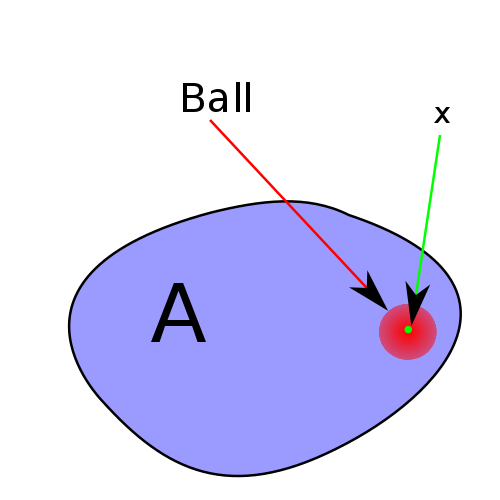
\includegraphics[width=0.45\textwidth]{img/openset}
      \caption{Quelle: Wikipedia}
\end{figure}

 \end{frame}


\begin{frame}
    \frametitle{Borelle'sche  $\sigma$-Algebra}
\framesubtitle{}
\begin{block}{Borellsche $\sigma$-Algebra}
Die Borel'sche   $\sigma$-Algebra über $\mathbb{R}^n$ ist die kleinste  $\sigma$-Algebra, die alle offenen Mengen $\mathcal{U}$ enthält, also 
\begin{align*}
A_\sigma (\mathcal{U}) := \bigcap \{  \mathcal{A} \subset \mathcal{P}(\mathbb{R}^n);  \;   \mathcal{U}  \subset  \mathcal{A},  \;  \mathcal{A} \text{ ist $\sigma$-Algebra} \}
\end{align*}
\end{block}

\begin{block}{Borellsche $\sigma$-Algebra existiert}
Die Borel'sche   $\sigma$-Algebra existiert, da die Potenzmenge eine   $\sigma$-Algebra ist.
\end{block}
\begin{block}{Borellsche $\sigma$-Algebra is Lebesgue messbar}
Die Borel'sche   $\sigma$-Algebra ist in der $\sigma$-Algebra der Lebesgue messbaren Mengen enthalten.
\end{block}
 \end{frame}



\begin{frame}
    \frametitle{Integration}
\framesubtitle{}

\begin{block}{Indikatorfunktion}
Für eine Menge $A \in \mathcal{A}$ einer $\sigma$-Algebra heißt
\begin{align*}
1_A(x) : = \begin{cases}
1 \text{ falls } x \in A
\\  0 \text{ sonst}
\end{cases}
\end{align*}
die Indikatorfunktion der Menge $A$.
\end{block}
 \end{frame}

\begin{frame}
    \frametitle{Inegration}
\framesubtitle{}
\begin{block}{Integration}
Für eine reelle Zufallsvariable $X: \Omega \to \mathbb{R}$ existiert eine endliche Reihe $s_n(x) := \sum_{i = 1}^{n} c_i \cdot 1_{A_j}$, so dass $s_n(x) \leq X(x)$ und  $\lim_{n \to \infty}  s_n(x) \to X(x)$ für alle $x \in \Omega$.
Man nennt $s_n$ auch einfache Funktion. Für eine einfache Funktion definiere
\begin{align*}
\int_\Omega s_n(x) \;  d\mu = \sum_{i=1}^{n} c_i \; \mu(A_i)
\end{align*}
\end{block}
\begin{block}{Integration}
Für eine positive, reelle Zufallsvariable $X: \Omega \to [0, \infty]$ definiere
\begin{align*}
\int_\Omega X \;  d \mu = \sup( \int_\Omega s_n(x) \;  d\mu ; s_n(x) \text{ einfach mit } s_n(x) \leq X(x))
\end{align*}
\end{block}
 \end{frame}



\begin{frame}
    \frametitle{Inegration}
\framesubtitle{}

\begin{block}{Integration}
Für allgemeines $X$ zerlege $X = X^+ - X^-$ mit $X^+ := \max(0, X)$ und $X^- := -min(0, X)$ und definiere 
\begin{align*}
\int_\Omega X(x) \;  d\mu  = \int_\Omega X^+(x) \;  d\mu - \int_\Omega X^-(x) \;  d\mu
\end{align*}

\end{block}


 \end{frame}



\begin{frame}
    \frametitle{Inegration}
\framesubtitle{}

\begin{block}{Integration}
\begin{align*}
\int_\Omega 1_A \; d\mu = \mu(A) 
\end{align*}
\end{block}
 \end{frame}




\begin{frame}
    \frametitle{Inegration}
\framesubtitle{}

\begin{block}{Satz von Fubuni}
Ist $f:  X  \times Y \to \mathbb{R}$ messbar und integrierbar, so ist 
\begin{align*}
\int_{ X  \times Y} f (x,y) \;  d(x,y) =  \int_Y \int_X  f(x,y) \; dx \; dy
\end{align*}
\end{block}
 \end{frame}


\begin{frame}
    \frametitle{Integration}
\framesubtitle{}

    \begin{block}{Beispiel}
$A:= \{ (x,y) \in \mathbb{R}^2 \;  | \;  x^2 + y^2 \leq 1\}$ (Kreisscheibe). $A_x =  \{ y  \in \mathbb{R} \;  | \; -1 \leq y \leq 1\} $
$A_y =  \{ x  \in \mathbb{R} \;  | \;  -\sqrt{1 - y^2} \leq x \leq \sqrt{1 - y^2} \} $
\end{block}
\begin{figure}[htp]
      \centering
    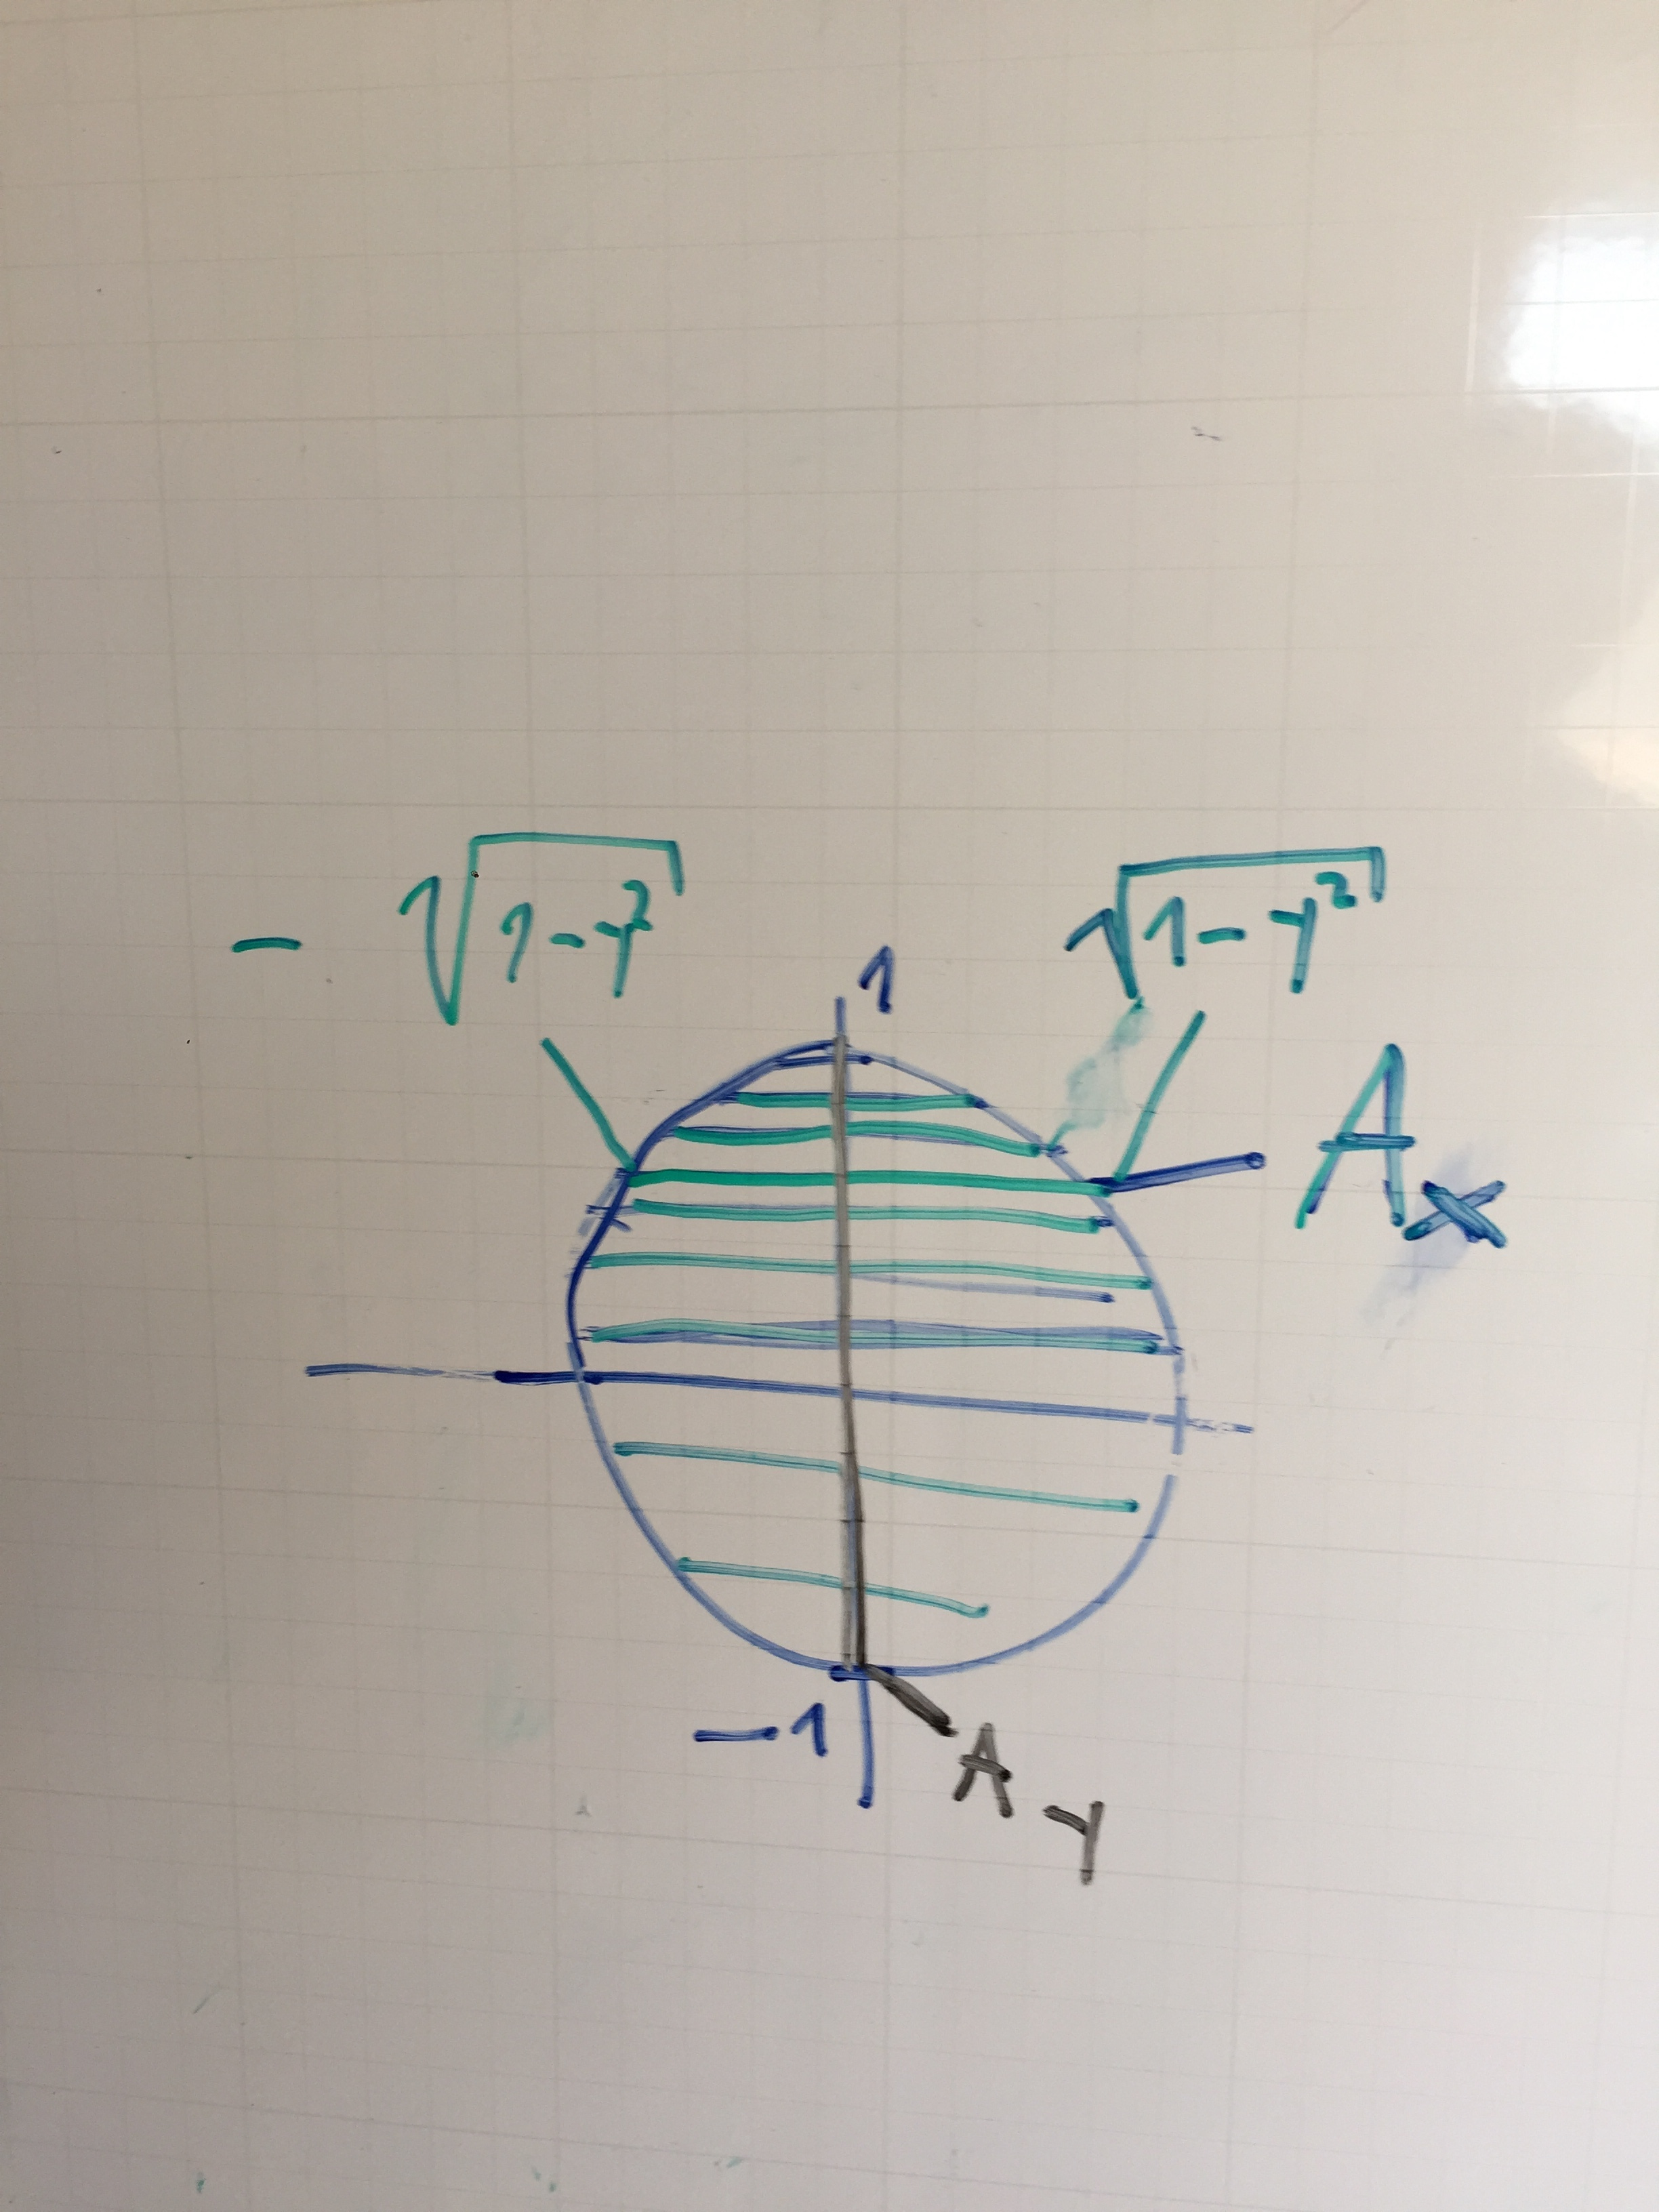
\includegraphics[width=0.35\textwidth]{img/int}
      \caption{Scheibenmengen}
\end{figure}
 \end{frame}

\begin{frame}
    \frametitle{Integration}
\framesubtitle{}

    \begin{block}{Beispiel}
\begin{align*}
\mu(A) = & \int_A 1  \; d(x,y) \;  := \int_{-1}^{1} \Biggl( \int_{-\sqrt{1 - y^2} }^{\sqrt{1 - y^2} } 1 \;  dx \Biggr) \; dy \\ 
& =  2 \int_{-1}^{1}  \sqrt{1 - y^2}   \; dy  \\ 
 & (substitution \;   y = sin(u)) =   2 \int_{-\frac{\pi}{2}}^{\frac{\pi}{2}}   \cos(u)^2   \; du = 2 \cdot \frac{\pi}{2} = \pi
\end{align*}
\end{block}

 \end{frame}










\end{document}
